\documentclass{article}
\usepackage{microtype}
\usepackage{graphicx}
\usepackage{subcaption}
\usepackage{booktabs}
\usepackage{seqsplit}
\usepackage{hyperref}
\newcommand{\theHalgorithm}{\arabic{algorithm}}
% Official, unmodified ICML 2026 initial anonymous submission style.
\usepackage{icml2026}
\usepackage{amsmath}
\usepackage{amssymb}
\usepackage{mathtools}
\usepackage{amsthm}
\usepackage[capitalize,noabbrev]{cleveref}
\newcommand{\tr}{\operatorname{tr}}
\newcommand{\RMSE}{\operatorname{RMSE}}
\newcommand{\MSE}{\operatorname{MSE}}
\newcommand{\E}{\mathbb{E}}
\newcommand{\Cov}{\operatorname{Cov}}
\icmltitlerunning{An Empirical Audit of Gaussian Benchmark Acquisition}

\begin{document}
\twocolumn[
\icmltitle{Predicting Unmeasured Benchmark Scores:\\
An Empirical Audit of Gaussian Trace-Risk Acquisition}
\begin{icmlauthorlist}
\icmlauthor{Anonymous Authors}{anon}
\end{icmlauthorlist}
\icmlaffiliation{anon}{Anonymous Institution}
\icmlcorrespondingauthor{Anonymous Authors}{anonymous@example.invalid}
\icmlkeywords{benchmark evaluation, missing data, Gaussian prediction, experimental design}
\vskip 0.3in
]
\printAffiliationsAndNotice{}

\begin{abstract}
Can a small set of whole benchmark tasks support prediction of a new model's unmeasured scores when historical evaluations are incomplete? We conduct a controlled empirical audit of standard Gaussian conditional prediction and greedy trace-risk acquisition, not a new acquisition algorithm. The primary panel contains 29 MTEB tasks and 278 embedding models, with 60 complete models in 19 conservative owner/adaptation components. On the designated split, measuring eight tasks yields group-macro full-suite RMSE 2.62 versus 4.01 for random acquisition with the same predictor; unmeasured-task RMSE is 3.08 versus 4.72. Trace-risk improves on random acquisition in all five overlapping splits, but comparisons with other selectors do not establish unique superiority. With six test components, the exact two-sided test cannot attain the first Holm threshold for eight comparisons. Numerical robustness is also limited: 18 of 33 executable Gaussian stress fits reach the 200-iteration cap, and two sparse-history conditions are infeasible. No evaluated non-full budget satisfies the illustrative validation adequacy rule on MTEB. A secondary six-task generative-model panel is reported as post-review exploratory corrective reanalysis after repairing a metadata-grouping defect, with unresolved data-license status. These results separate acquisition benefits, unseen-score prediction, and the limits of conditional uncertainty estimates.
\end{abstract}

\section{Introduction}
\label{sec:intro}
Evaluating a new model on every task in a benchmark suite may be undesirable, but replacing measurements with predictions changes what an evaluation establishes. Correlation across historical scores can make prediction useful; it cannot by itself show that a particular small budget is adequate. Historical result matrices add a second difficulty: different models have been evaluated on different tasks, and availability can depend on performance or developer choices.

We study a precise acquisition problem. A budget buys complete task evaluations, not individual examples. A fixed, offline ordering chooses which tasks to measure for a new model; those exact scores are then used to predict the rest of a frozen panel. The historical matrix is incomplete, while evaluation targets are complete held-out models. We audit a standard combination of missing-data Gaussian estimation, conditional-mean prediction, and greedy reduction of residual covariance trace. The contribution is the controlled empirical assessment, including its failures, rather than algorithmic novelty, priority, or a state-of-the-art claim.

Two distinctions determine the interpretation. First, full-suite reconstruction credits the exact measurements themselves. Prediction on unmeasured tasks is the practical target, but at equal budget its MSE is a deterministic rescaling of full-suite MSE; it is not independent corroboration. Comparing methods on tasks that neither measured supplies a complementary, pair-specific diagnostic. Second, many model rows do not imply many independent evaluation units. We split conservative owner/adaptation components, without claiming that available metadata completely identifies model ancestry.

The primary experiment uses 29 English MTEB tasks across seven task types. Its 60 complete anchor models span only 19 components. We therefore emphasize effect sizes and split sensitivity: the six-component designated test split is structurally unable to reject any of eight Holm-corrected exact comparisons. We also make a numerical failure prominent: most executable stress fits do not meet the estimator's stopping criterion. Neither a finite error table nor convergence of the main fits establishes robustness of the converged estimator under sparse history.

The study addresses three questions: does trace-risk acquisition improve on random queries with a matched predictor; how much of the apparent benefit persists on shared unmeasured targets; and can a validation-only rule identify an adequate budget? The answers are conditional. Point reconstruction improves over random acquisition, but simple selectors can be competitive. The declared MTEB adequacy rule returns no non-full budget. Our secondary OpenLLM analysis is a post-review exploratory corrective reanalysis on a distinct small suite, not pristine confirmatory or license-cleared replication.

\section{Related Work and Scope}
\label{sec:related}
MTEB documents heterogeneous embedding applications and the absence of a single model dominating all task types \citep{muennighoff2022mteb}. We use a frozen historical subpanel, not the full benchmark or a current leaderboard. Differences between task metrics remain relevant even after their scores are put on a common numerical scale.

Reducing examples within tasks is distinct from choosing whole tasks. tinyBenchmarks selects example anchors using historical responses and item-response representations, then reconstructs benchmark scores \citep{polo2024tinybenchmarks}. metabench combines item-level reduction with cross-benchmark calibration, retaining selected items from all six source benchmarks \citep{kipnis2024metabench}. These studies motivate economical evaluation, but their test-time inputs and budgets differ from ours. We do not relabel their item selectors as whole-task baselines or compare incompatible published errors.

Observational Scaling Laws predicts downstream performance from measured benchmark scores through low-dimensional capabilities; its experimental-design application selects model/family rows, not task columns \citep{ruan2024observational}. Sloth instead connects resource variables and family-specific calibration to shared skills and multi-benchmark performance \citep{polo2024sloth}. Our predictor uses acquired scores, not parameter or token counts. Low-dimensional structure motivates testing score prediction, but is not a guarantee of adequate acquisition.

This discussion is deliberately restricted to five directly read, allowlisted papers. It is not a comprehensive review and supports no claim of first use. We use standard Gaussian and linear-prediction identities, deriving them in \cref{app:identities} rather than presenting them as new theorems. The source-access boundaries are recorded in \cref{app:sources}.

\section{Prediction and Acquisition}
\label{sec:method}
\subsection{Problem and evaluation target}
Let $X\in\mathbb{R}^p$ contain a new model's task scores. Historical rows reveal arbitrary subsets. An offline policy selects $S\subseteq\{1,\ldots,p\}$ with $|S|=k$, then a predictor observes only $X_S$. Queries have equal assumed cost and return exact scores. There is no adaptation to the new model's observed values, no benchmark-noise model, and no measured evaluation-time saving.

For complete test rows $i$ in components $g=1,\ldots,G$, with $n_g$ rows in component $g$, define
\begin{align}
 L_g(S)&=\frac{1}{n_gp}\sum_{i\in g}\sum_{j=1}^p(\widehat X_{ij}-X_{ij})^2,\label{eq:metric}\\
 R_{\rm full}&=\sqrt{\frac1G\sum_g L_g(S)}.\nonumber
\end{align}
Thus groups and tasks receive equal weight, after averaging rows within group. This is a square root of macro MSE, not an average of group RMSEs. Observed coordinates are copied exactly. On $U=S^c$, the analogous unseen endpoint satisfies, for every $k<p$,
\begin{equation}
 \MSE_{\rm unseen}=\frac{p}{p-k}\MSE_{\rm full}.
 \label{eq:unseen}
\end{equation}
It measures the actual omitted-score error, but the target set varies with the selector. We also evaluate a pair of policies on $\{1,\ldots,p\}\setminus(S_A\cup S_B)$ and report the number of shared unseen tasks. Such intersections differ across pairs and do not form one common-target ranking.

\subsection{Standard conditional prediction and greedy trace reduction}
For Gaussian $X$ with mean $\mu$ and positive-definite covariance $\Sigma$, the conditional mean and residual covariance are
\begin{align}
 \widehat X(S)&=\mu+\Sigma_{:S}\Sigma_{SS}^{-1}(X_S-\mu_S),\label{eq:predict}\\
 C(S)&=\Sigma-\Sigma_{:S}\Sigma_{SS}^{-1}\Sigma_{S:}.\label{eq:conditional}
\end{align}
The Gaussian squared-error risk is $\tr C(S)/p$. Without Gaussianity these formulas characterize the best affine predictor under the stated second moments, not necessarily the conditional expectation or conditional covariance.

Starting at $S=\varnothing$, trace-risk acquisition selects the unqueried coordinate with largest unnormalized gain
\begin{align}
 \Delta_j(S)&=\frac{\|C(S)_{:j}\|_2^2}{C(S)_{jj}},\label{eq:gain}\\
 C&\leftarrow C-\frac{C_{:j}C_{j:}}{C_{jj}}.\nonumber
\end{align}
The corresponding normalized risk gain is $\Delta_j/p$. It includes the benefit of directly measuring coordinate $j$. Gaussian conditional covariance does not depend on the realized query values, so this policy is an offline ordering. We use linear solves, not explicit inverses. Trace reduction is monotone, but is \emph{not generally submodular}; \cref{app:counterexample} supplies a positive-definite three-variable counterexample. We claim neither global optimality nor a generic submodular approximation guarantee.

\subsection{Fitting incomplete history}
Training rows receive weights $w_i=1/(G_{\rm tr}n_{g(i)})$. Observed-entry weighted means and standard deviations define training-only standardization, with a one-score-point SD floor. Gaussian fitting alternates conditional sufficient-statistic updates with diagonal covariance shrinkage in standardized coordinates and a $10^{-6}$ eigenvalue floor. Shrinkage is applied at every update, so this is a regularized fixed-point estimator, not an unqualified unpenalized maximum-likelihood fit. The final cap is 200 updates and the relative-change tolerance is $10^{-5}$. Entirely unobserved training tasks cause failure rather than an invented mean. We do not identify the mechanism of historical missingness; in particular, ordinary observed-data fitting is not a correction for nonignorable reporting.

We compare prediction mechanisms using an observed-entry ridge factor model. Its alternating least-squares (ALS) updates use group weights; zero filling is only an SVD initialization, never the fitted loss. ALS runs for 40 fixed steps, without a global convergence claim. At test time latent coefficients are inferred from the queried scores. Details and computational bounds appear in \cref{app:implementation}. All models use only the acquired coordinates of a target row.

\section{Experimental Protocol}
\label{sec:experiments}
\subsection{Data, grouping, and quality control}
The primary source is the pinned CC0 MTEB results snapshot described in \cref{app:data}. A prespecified list of 32 English tasks is reduced using availability and component coverage, not score magnitudes. Dropping three tasks gives the first feasible panel: 278 models, 29 tasks, 60 complete models, 19 complete-anchor components, and 74 components overall. The observed fraction is 64.71\%. ``Full suite'' always means these 29 tasks, not all MTEB.

Parsing keeps eligible English test-split native main scores, converts fractions to score points, fixes a modal dataset revision per task by availability, and chooses model revisions by coverage with deterministic revision ties. Missing and rejected records are not zeros. Exact duplicate score/mask rows are checked; none are removed from the primary candidate matrix. These checks do not establish freedom from near-duplicates, training contamination, or evaluator-version heterogeneity. \Cref{fig:missingness} displays the remaining missingness.

\begin{figure}[t]
\centering
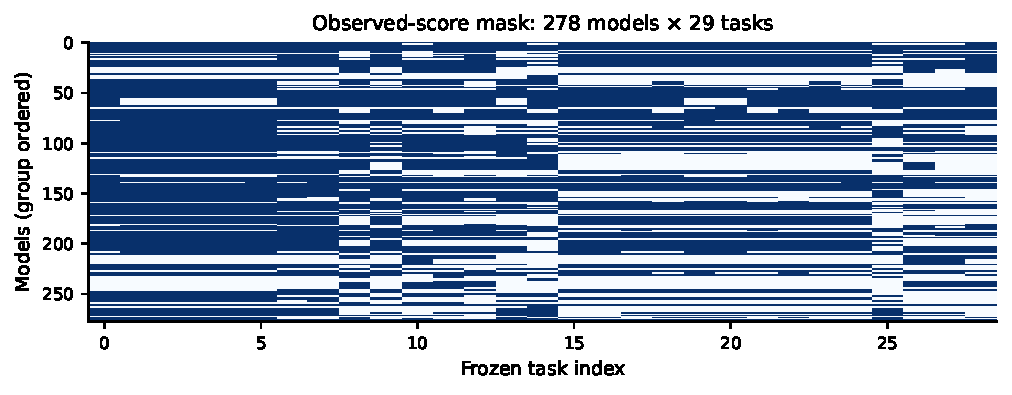
\includegraphics[width=\columnwidth]{figures/missingness.pdf}
\caption{Observed-score mask for the frozen MTEB panel, with rows ordered by component. Blue denotes observed scores. Complete anchors define evaluation targets; incomplete histories enter training only when their component is assigned to training.}
\label{fig:missingness}
\end{figure}

Components unite same-owner models and explicit adaptation/base edges, including shared external bases. Owners are repository namespaces; 199 of 278 MTEB adaptation fields are missing, and three absolute local paths supply no usable ancestry edge. Missing-value sentinels (including \texttt{Removed}) add no edges. They are conservative metadata components, not certified independent model families or a complete ancestry reconstruction. For each seed $11,23,37,53,71$, seven anchor components train, six validate, and six test. Non-anchor-only components are assigned approximately 60/20/20; their incomplete rows are retained only in training. No row from a held-out component contributes historical training scores. Split 11 has 118 training rows, 18 complete validation rows, and 23 complete test rows; \cref{tab:splits} gives all memberships' counts.

The secondary OpenLLM panel contains 3,748 complete models in 472 owner/base components on six raw-score tasks. It excludes records marked flagged or merged, resolves model duplicates deterministically, and removes identical score rows. Components split into 282/95/95 training/validation/test groups; split 11 has 478 test rows. This source's dataset license is unspecified. We retain that uncertainty, do not propose raw-data relicensing, and keep this complete-history generative-model analysis separate from the incomplete-history embedding experiment.

\subsection{Stages, tuning, and comparisons}
The study proceeds through panel/split freezing, bounded training/validation tuning, fixed-budget testing, history stress tests, and validation-selected budget auditing. Success means an auditable estimate or an explicitly logged failure, not necessarily a positive result. The prospective protocol and implementation deviations are preserved; they are not an external preregistration. A first run exposed a serialization error, capped fits, and audit issues; the final run uses the corrected independent task-mean baseline, uniform 200-step Gaussian cap, and expanded adequacy multiplicity accounting. Pilot outputs are excluded (\cref{app:reproduction}).

\paragraph{Post-review repair.} Independent self-review found that 549 retained OpenLLM \texttt{Base Model} fields contained \texttt{Removed}, which the graph incorrectly treated as a common ancestor. The repair normalizes known missing-value sentinels to missing before adding edges, preserving valid slash-free identifiers. Secondary components change from 381 to 472; both score matrices and the MTEB panel/groups remain byte-identical. All experiments, including secondary tuning, acquisition, adequacy, and inference, were rerun with the same seeds, grids, and metric protocol. We withdraw the old secondary conclusions. Because results had already been inspected, the corrected secondary analysis is \emph{post-review exploratory corrective reanalysis}, not pristine confirmatory replication; the full chronology and archived flawed outputs are identified in \cref{app:reproduction}.

The main MTEB budgets are $\{0,1,2,4,8,14,29\}$, with $k^*=\lceil p/4\rceil=8$ fixed for the designated comparison. OpenLLM uses $\{0,1,2,3,4,6\}$ and $k^*=2$. Gaussian shrinkage is selected from $\{0.1,0.3,0.6,0.9\}$; factor ranks are $\{2,4,8\}$ clipped to feasible dimensions, and ridge penalties are $\{0.01,0.1\}$. Tuning minimizes validation full-suite MSE averaged over nontrivial budgets and the first five shared random paths. Evaluation averages losses over 20 nested random permutations, never predictions. Transforms and fitted parameters use training data only; validation is not absorbed into training. Hyperparameters, orders, and adequacy policies are written before test errors are computed.

Eight comparisons isolate selector and predictor effects: random queries plus Gaussian prediction; descending raw marginal variance; static absolute-correlation centrality; greedy maximum entropy (conditional-variance/log-determinant selection); training-inner out-of-fold (OOF) greedy error minimization; random queries plus observed task means; random queries plus factors; and Gaussian trace-risk queries plus factors. All covariance selectors share the tuned Gaussian fit. Maximum entropy is a determinant-design proxy, not a general parameter-information guarantee. OOF uses three grouped folds and complete training anchors as targets, retaining available histories from other training components. Its shrinkage comes from outer validation, so it is not fully nested tuning. Two of its 30 inner fits reach the cap, limiting this comparator's numerical interpretation.

\subsection{Uncertainty and inference}
Split 11 is the designated inferential comparison; remaining overlapping splits assess sensitivity and are not independent replications. We compare paired component-level MSEs, first averaging random-path losses. Two-sided sign-randomization tests require the stated symmetry/exchangeability of component differences; component metadata do not guarantee that assumption. MTEB enumerates all signs. OpenLLM uses 10,000 Monte Carlo signs with the plus-one correction. Holm correction covers eight comparisons separately within each dataset. Other budgets and stresses are exploratory.

Tables report 2,000-draw component-block percentile bootstrap intervals conditional on fixed fits and policies. They omit training, task-panel, and lineage uncertainty; marginal 95\% intervals are not multiplicity-adjusted. Across-seed ``$\pm$'' is the sample SD of overlapping splits, \emph{not} a confidence interval. Crucially, six MTEB test groups give minimum exact two-sided $p=2/2^6=0.03125$, exceeding Holm's first threshold $0.05/8=0.00625$. No rejection is attainable in this design, regardless of effect size. Nonsignificance therefore does not establish equivalence.

\section{Results}
\label{sec:results}
\begin{table*}[t]
\caption{Group-macro full-suite RMSE in score points (lower is better), at MTEB $k=8$ and secondary OpenLLM $k=2$. Brackets are marginal 95\% test-component bootstrap intervals conditional on fixed fits; five-split summaries are mean $\pm$ overlapping-split SD, not confidence intervals. Queried entries have zero error. No MTEB Holm-corrected rejection is attainable with six test components. OpenLLM entries use the repaired graph and are post-review exploratory results.}
\label{tab:main}
\centering
\resizebox{\textwidth}{!}{\begin{tabular}{lrrrr}
\toprule
Method & MTEB: split 11 & MTEB: five splits & OpenLLM: split 11 & OpenLLM: five splits \\
\midrule
Trace-risk & 2.62 [1.93, 3.18] & 3.32 $\pm$ 0.93 & 3.93 [3.46, 4.43] & 4.17 $\pm$ 0.24 \\
Random + Gaussian & 4.01 [3.22, 4.67] & 4.65 $\pm$ 0.80 & 6.42 [5.92, 6.90] & 6.72 $\pm$ 0.30 \\
Marginal variance & 3.33 [1.90, 4.57] & 3.72 $\pm$ 0.84 & 4.56 [4.12, 5.01] & 4.64 $\pm$ 0.20 \\
Correlation centrality & 4.11 [3.24, 4.88] & 4.81 $\pm$ 0.69 & 6.88 [6.23, 7.53] & 7.11 $\pm$ 0.51 \\
Max. entropy & 2.75 [2.05, 3.43] & 3.53 $\pm$ 0.99 & 4.56 [4.12, 5.01] & 4.64 $\pm$ 0.20 \\
OOF-greedy & 2.78 [2.28, 3.26] & 3.53 $\pm$ 0.84 & 3.93 [3.46, 4.43] & 4.17 $\pm$ 0.24 \\
Random + task mean & 11.92 [8.43, 14.84] & 12.04 $\pm$ 2.30 & 9.43 [8.65, 10.17] & 10.02 $\pm$ 0.38 \\
Random + factor & 4.79 [4.05, 5.44] & 5.28 $\pm$ 0.69 & 9.21 [8.60, 9.81] & 9.64 $\pm$ 0.80 \\
Trace-risk + factor & 3.10 [2.45, 3.68] & 4.12 $\pm$ 1.01 & 4.13 [3.71, 4.56] & 4.51 $\pm$ 0.39 \\
\bottomrule
\end{tabular}
}
\end{table*}

\begin{figure*}[t]
\centering
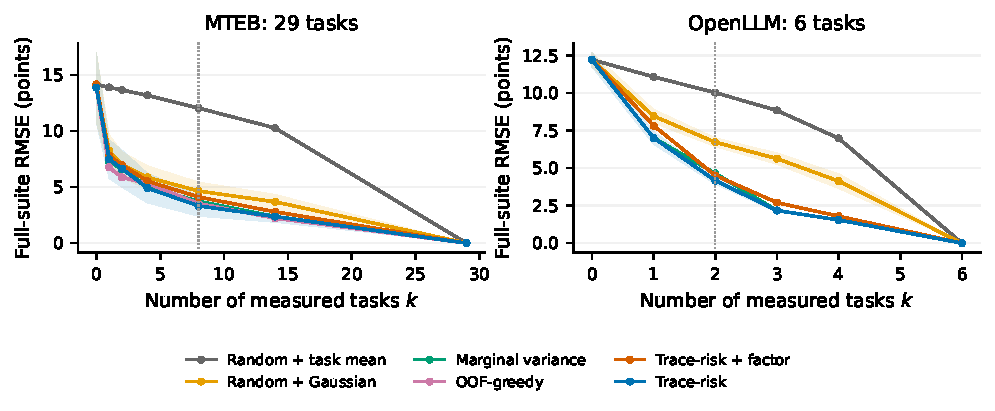
\includegraphics[width=\textwidth]{figures/risk_curves.pdf}
\caption{Full-suite RMSE versus measured task count, averaged across five overlapping splits. Shading shows one split SD for trace-risk and random Gaussian prediction, not inferential uncertainty. Vertical dotted lines mark the fixed comparison budgets. The zero-error $k=p$ endpoint measures every score; it provides no evidence of prediction quality on unseen tasks. OpenLLM uses the repaired grouping in a post-review exploratory reanalysis of a distinct population.}
\label{fig:curves}
\end{figure*}

\subsection{Matched-budget reconstruction and unseen scores}
The tuned MTEB training covariance has median off-diagonal correlations ranging from 0.653 to 0.696 across the five splits, and raw-covariance effective rank $\exp[-\sum_j q_j\log q_j]$ of 4.26--4.61, where $q_j$ are normalized eigenvalues. These are shrinkage-model summaries of the historical scores, not unbiased population correlations or a prediction guarantee; their per-split values are saved in \texttt{train\_correlations.csv}.

Trace-risk improves point reconstruction over random acquisition with the same Gaussian predictor (\cref{tab:main}). On MTEB split 11, full-suite RMSE is 2.62 [1.93, 3.18] versus 4.01 [3.22, 4.67]. The paired RMSE difference is $-1.39$ points, with marginal interval $[-2.20,-0.83]$. This interval is descriptive conditional evidence, not a rejection of the multiplicity-controlled primary null: raw $p=0.03125$ and Holm $p=0.25$ (\cref{tab:inference}).

Across five overlapping MTEB splits, trace-risk is 3.32 $\pm$ 0.93 versus 4.65 $\pm$ 0.80 for random Gaussian prediction. Its point error is lower in all five, but not uniformly lower than every selector: maximum entropy is lower on seed 53 and OOF-greedy on seed 71. The small designated-split gaps to maximum entropy (2.75) and OOF-greedy (2.78) do not establish unique superiority. \Cref{fig:curves,tab:perseed} expose budget and split dependence.

The primary practical endpoint is omitted-score prediction. On split 11, MTEB unseen RMSE is 3.08 for trace-risk and 4.72 for random Gaussian acquisition. These follow exactly from multiplying each full-suite RMSE by $\sqrt{29/21}$; they are not another independent experiment. Pairwise common-unseen evaluation is more revealing: against random Gaussian acquisition, trace-risk is 3.08 versus 3.36 on an average of 15.3 shared unseen tasks (\cref{tab:common}). This smaller gap is consistent with a contribution from direct measurement and changed target composition. The diagnostic does not causally decompose that advantage and has a different target intersection for each pair.

Predictor quality matters alongside selection. On MTEB split 11, random queries with task means yield 11.92, versus 4.01 with Gaussian prediction and 4.79 with factors. Sharing trace-risk queries reduces factor RMSE to 3.10, but it remains above the matched-query Gaussian value 2.62. These are controlled comparisons within this panel, not rankings against methods from unlike evaluation regimes.

In the corrected, post-review exploratory OpenLLM analysis, split-11 trace-risk gives 3.93 [3.46, 4.43] versus random Gaussian 6.42 [5.92, 6.90]; unseen RMSE is 4.82 versus 7.86. Marginal variance and maximum entropy both give 4.56, while OOF-greedy matches 3.93 exactly. Trace-risk is better than random in all five splits (4.17 $\pm$ 0.24 versus 6.72 $\pm$ 0.30), not uniquely best among selectors. The secondary eight-way corrected comparison with random has Monte Carlo Holm $p\approx0.0008$; variance/maximum entropy give Holm $p=0.137$, and OOF gives $p=1$. This does not repair the primary study's resolution or establish broad generative-model transfer.

\subsection{Sparse-history stress: capped algorithms, not converged robustness}
\label{sec:stress}
\textbf{Numerical failure is a central result.} All ten selected main Gaussian fits satisfy the stopping rule. In contrast, 18 of 33 executable MTEB stress fits fail to reach tolerance by 200 iterations, and two additional conditions are infeasible because a task has no observations (MCAR 20\%, seeds 23 and 53). We neither resample these failures nor silently discard capped predictions. \Cref{tab:stress} describes the \emph{200-step capped algorithm}, not robustness of a converged estimator. The executable denominators and convergence counts are explicit in \cref{tab:convergence}.

\begin{table*}[t]
\caption{Exploratory MTEB stress/ablation full-suite RMSE at $k=8$, mean $\pm$ overlapping-split SD (lower is better). \textbf{18/33 executable Gaussian fits are nonconverged at the 200-step cap.} MCAR 20\% additionally fails on seeds 23 and 53, leaving only three executable splits. ``Factor'' uses each condition's Gaussian trace-risk queries. Complete-history/masked conditions use only complete training anchors; diagonal and no-shrinkage conditions use natural training histories. These different cohorts preclude attributing a natural-history versus complete-history gap solely to missingness.}
\label{tab:stress}
\centering
\resizebox{\textwidth}{!}{\begin{tabular}{lrrrrrr}
\toprule
History / ablation & Trace-risk & Random & Variance & Max. entropy & Factor & Splits \\
\midrule
Complete history & 4.01 $\pm$ 0.45 & 5.22 $\pm$ 0.56 & 4.05 $\pm$ 0.71 & 4.01 $\pm$ 0.62 & 4.22 $\pm$ 0.69 & 5 \\
MCAR 50\% & 4.91 $\pm$ 0.80 & 6.40 $\pm$ 0.36 & 4.79 $\pm$ 0.26 & 4.86 $\pm$ 0.46 & 5.63 $\pm$ 0.56 & 5 \\
MCAR 20\% & 9.00 $\pm$ 0.42 & 23.05 $\pm$ 12.08 & 8.82 $\pm$ 0.67 & 8.99 $\pm$ 0.43 & 11.45 $\pm$ 1.39 & 3 \\
MNAR high-favored & 5.33 $\pm$ 1.55 & 7.84 $\pm$ 2.01 & 5.58 $\pm$ 1.98 & 5.29 $\pm$ 1.54 & 6.00 $\pm$ 1.66 & 5 \\
MNAR low-favored & 6.35 $\pm$ 0.98 & 8.52 $\pm$ 1.69 & 6.16 $\pm$ 0.76 & 6.32 $\pm$ 0.93 & 7.55 $\pm$ 1.22 & 5 \\
Diagonal covariance & 9.44 $\pm$ 2.21 & 12.04 $\pm$ 2.30 & 9.44 $\pm$ 2.21 & 9.44 $\pm$ 2.21 & 5.34 $\pm$ 1.46 & 5 \\
No shrinkage & 3.86 $\pm$ 0.90 & 5.33 $\pm$ 1.05 & 4.33 $\pm$ 0.95 & 4.10 $\pm$ 1.10 & 4.34 $\pm$ 1.04 & 5 \\
\bottomrule
\end{tabular}
}
\end{table*}

\begin{figure*}[t]
\centering
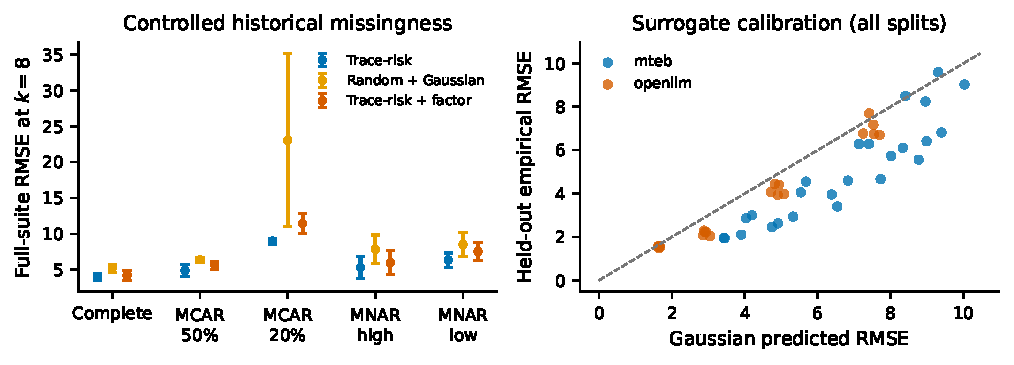
\includegraphics[width=\textwidth]{figures/stress_calibration.pdf}
\caption{Left: controlled-history errors, with split SD bars and only three executable MCAR-20\% splits; capped, nonconverged fits remain included (\cref{sec:stress}). Right: fitted Gaussian predicted full-suite RMSE versus held-out empirical RMSE across nonzero, non-full budgets and splits. The dashed diagonal denotes equality, not a confidence bound. These descriptive diagnostics are not robustness or coverage certificates.}
\label{fig:stresscal}
\end{figure*}

Masks act only on complete training anchors, preserving each split's test cohort and main hyperparameters. MCAR retains cells independently with nominal probability 1, 0.5, or 0.2. High-/low-favored MNAR masks use logistic slopes $+1.5/-1.5$ on complete-training-anchor scores standardized using unweighted column means and population SDs (floored at one), with an intercept calibrated to 50\% \emph{expected} retention, not exactly 50\% realized retention. Empty rows convey no observed information and are removed. Realized retention and pair support are reported in \cref{tab:convergence}.

Within this capped procedure, trace-risk RMSE rises from 4.01 with complete-anchor histories to 4.91 under MCAR 50\% and 9.00 among executable MCAR 20\% conditions. MNAR high-/low-favored histories yield 5.33/6.35. Other selectors sometimes match or improve on these point errors. Zero pair support in some masks further limits covariance identification. Diagonal covariance gives 9.44, while the no-shrinkage point value 3.86 is based on five nonconverged fits and cannot establish superiority of an unregularized converged estimator. Natural incomplete-history versus complete-anchor comparisons also change row composition and sample size, so they do not isolate a benefit from missingness.

\subsection{Model uncertainty and validation-only adequacy}
\label{sec:adequacy}
Model-implied covariance is not empirically calibrated uncertainty (\cref{fig:stresscal}). At the fixed MTEB budget, mean predicted RMSE is 5.24 versus empirical 3.32; nominal 90\% marginal unseen intervals have group-macro coverage 0.974, ranging from 0.939 to 0.997 across splits. Corrected OpenLLM gives 4.89 versus 4.17 and coverage 0.934, ranging from 0.921 to 0.945 (\cref{tab:calibration}). Such overcoverage at these budgets does not establish a valid guarantee under shift or over all tasks. At $k=0$, two MTEB splits have coverage near 0.83, illustrating budget dependence. A 50,000-draw, 12-task Gaussian simulation checks the known-parameter risk calculation to maximum relative discrepancy 0.0065; this checks theory/implementation, not Gaussianity of leaderboard data.

Our adequacy policy chooses the smallest evaluated $k<p$ whose validation upper bounds meet both illustrative tolerances: two points full-suite RMSE and three points unseen RMSE. It requires at least six validation components and uses 2,000 component-bootstrap draws at one-sided percentile quantile $1-0.05/(4B\cdot2)$, accounting for four shrinkages, $B$ candidate budgets, and two endpoints. At fixed $k$ the endpoints remain algebraically dependent. Including zero and excluding full measurement gives $B=6$ for MTEB and $B=5$ for OpenLLM: only about 2.1--2.5 of the 2,000 bootstrap draws lie beyond the nominal tail quantile. This poorly resolved Bonferroni-tail heuristic does not turn a conditional, small-group percentile procedure into a 95\% certificate; tuning reuse, training uncertainty, and distribution shift remain limitations.

No evaluated MTEB non-full budget qualifies on any split. This is a failure to validate adequacy, not proof that all possible budgets or policies are inadequate. On corrected OpenLLM the rule selects $k=4$ in two of five splits, seeds 23 and 53. Their frozen-policy test full-suite RMSEs are 1.59 and 1.56, with unseen RMSEs 2.75 and 2.70, respectively. Their marginal conditional intervals appear in \cref{tab:policytest}; these are not simultaneous post-selection guarantees. Smallest budgets passing test point tolerances are post-hoc only and confined to \cref{tab:adequacy}. There is no universal small-$k$ conclusion: even an isotropic Gaussian has unseen RMSE $\sigma$ for every $k<p$ (\cref{app:diagonal}).

\section{Discussion and Limitations}
\label{sec:discussion}
The evidence supports a restricted empirical observation: covariance-aware prediction and selected queries can lower reconstruction error relative to random acquisition in these frozen panels. It does not establish a uniquely superior selector or reliable adequacy calibration. Conditional risk estimates omit mean/covariance shift and estimation uncertainty; \cref{app:shift} derives their exact second-moment decomposition. An apparent risk reduction can result partly from measuring high-variance tasks rather than transferring information to other tasks.

Generalization is constrained by coverage-biased complete anchors, imperfect owner/base metadata, seven training anchor components, heterogeneous main metrics, and unknown benchmark contamination. The generative-model panel has only six tasks, complete histories, unresolved license status, and post-review exploratory status after the grouping repair; it is not an independent confirmatory or license-cleared universal replication. OOF cap failures and widespread stress nonconvergence are numerical defects of the evaluated bounded procedure, not just population-scope caveats. Factor objective monitoring does not establish a global optimum. Row-random diagnostics, if consulted in the artifacts, also change cohorts, weights, and sample counts and cannot identify a causal leakage effect.

A future confirmatory design needs more independent groups, a separate tuning/calibration allocation, and predeclared training-only convergence gates. At least nine nonzero independent paired groups are needed merely to make the present eight-way exact Holm rejection attainable, not to ensure power. Further work should model unequal evaluation costs and noisy measurements, test temporal/specialized populations, and investigate sparse-history identification before extending robustness claims. We report no measured benchmark-execution speedup: counting tasks is an assumed cost proxy, not wall-clock evidence.

\section{Conclusion}
\label{sec:conclusion}
This controlled audit finds lower point reconstruction error for standard Gaussian trace-risk acquisition than matched random queries across five overlapping splits, but not unique selector superiority. Actual unseen-score errors and pairwise common-unseen diagnostics qualify the acquisition benefit. Structural primary underpower, failed MTEB adequacy validation, and pervasive stress-fit nonconvergence prevent stronger claims. The deliverable is a reproducible account of where this standard pipeline helps and where its numerical and uncertainty assumptions remain insufficient, not a new algorithm or a universal small-budget evaluation guarantee.

% Flush the main-body floats before the separately required, uncounted section.
\clearpage
\section*{Impact Statement}
Predicting rather than measuring benchmark performance could reduce evaluation burden if validated for an intended use. It can also conceal specialized failures, amplify historical reporting bias, and encourage unsupported leaderboard or deployment claims. Our aggregate reconstruction endpoint does not certify safety, fairness, or any particular omitted task. Users should distinguish measured from predicted scores and rerun relevant tasks before consequential decisions. Public model-result metadata do not resolve benchmark contamination or all upstream rights. The primary results snapshot is CC0; the secondary dataset's license is unspecified and raw-data redistribution is not recommended. No new human-subject data, foundation-model training, paid inference, or GPU evaluation is involved in this audit. We make no measured environmental-benefit claim.

\bibliographystyle{icml2026}
\bibliography{references}

\clearpage
\appendix
\onecolumn
\section{Standard Prediction Identities and Their Boundaries}
\label{app:identities}
These derivations restate standard Gaussian conditioning and affine prediction facts. They are included to fix normalization, identify assumptions, and delimit the empirical claims; none is a novelty claim.

\subsection{Conditional covariance and squared-error risk}
Let $E_S$ select the queried coordinates, assume $\Sigma\succ0$, and put $B=\Sigma_{:S}\Sigma_{SS}^{-1}$. Define $e=X-\mu-B(X_S-\mu_S)$. Direct multiplication gives
\begin{align}
 \Cov(e,X_S)&=\Sigma_{:S}-B\Sigma_{SS}=0,\\
 \Cov(e)&=\Sigma-B\Sigma_{S:}-\Sigma_{:S}B^\top+B\Sigma_{SS}B^\top
 =\Sigma-\Sigma_{:S}\Sigma_{SS}^{-1}\Sigma_{S:}=C(S).
\end{align}
For jointly Gaussian $X$, the residual $e$ is jointly Gaussian with $X_S$ and uncorrelated with it, hence independent. Its mean is zero. Consequently $\E[X\mid X_S]=\mu+B(X_S-\mu_S)$ and $\Cov(X\mid X_S)=C(S)$. For any square-integrable predictor $g(X_S)$, write $X-g=e+(\E[X\mid X_S]-g)$. Conditional residual mean zero eliminates the cross term, yielding
\begin{equation}
 \frac1p\E\|X-g(X_S)\|^2
 =\frac1p\tr C(S)+\frac1p\E\|\E[X\mid X_S]-g(X_S)\|^2.
\end{equation}
Thus the conditional mean is Bayes-optimal under squared loss and has normalized risk $\tr C(S)/p$. Queried covariance rows/columns vanish. Empty queries give $C=\Sigma$; querying every coordinate gives $C=0$. These are true-moment statements, not coverage claims for a fitted covariance.

For a non-Gaussian distribution with finite second moments, the same residual orthogonality and covariance calculations hold. After optimizing the intercept, an affine predictor has the form $\mu+A(X_S-\mu_S)$. Orthogonality gives
\begin{equation}
 \frac1p\E\|X-\mu-A(X_S-\mu_S)\|^2
 =\frac{\tr C(S)}p+\frac{\tr[(A-B)\Sigma_{SS}(A-B)^\top]}p.
\end{equation}
Hence $B$ is best affine, but need not be the conditional mean. For example, $X=(Z,Z^2-1)$ for standard normal $Z$ has covariance $\operatorname{diag}(1,2)$. Querying $X_1$ leaves affine normalized risk 1, whereas the nonlinear predictor $X_2=X_1^2-1$ is exact. Gaussian Bayes language cannot be inferred from second moments alone.

\subsection{Rank-one update and the direct-measurement term}
After querying $S$, residualize candidate $j$ as $r_j=X_j-\widehat X_j(S)$. Its variance is $C_{jj}$ and $\Cov(e,r_j)=C_{:j}$. Adding the affine prediction based on $r_j$ gives residual $e'=e-C_{:j}r_j/C_{jj}$. Expansion gives
\begin{equation}
 C(S\cup\{j\})=C(S)-\frac{C_{:j}C_{j:}}{C_{jj}},\qquad
 \tr C(S)-\tr C(S\cup\{j\})=\frac{\|C_{:j}\|_2^2}{C_{jj}}.
\end{equation}
This is also Gaussian sequential conditioning. The normalized MSE reduction divides by $p$, not by the changing number of unmeasured tasks. The summand $C_{jj}^2/C_{jj}=C_{jj}$ is the variance removed by directly measuring the candidate. If $C_{jj}=0$, positive semidefiniteness forces $C_{:j}=0$; the gain is defined as zero. Positive-definite initial covariance avoids this degeneracy for unqueried coordinates in exact arithmetic.

\subsection{Trace reduction is not generally submodular}
\label{app:counterexample}
Let $U,V,W$ be independent standard Gaussians and $X=(U,U+V,2V+W)$. Its positive-definite covariance is
\begin{equation}
 \Sigma=\begin{pmatrix}1&1&0\\1&2&2\\0&2&5\end{pmatrix}.
\end{equation}
Positive definiteness follows because the linear transformation from $(U,V,W)$ is invertible. Querying coordinate 1 initially has trace gain $(1^2+1^2)/1=2$. After first querying coordinate 2,
\begin{equation}
 C(\{2\})=\begin{pmatrix}1/2&0&-1\\0&0&0\\-1&0&3\end{pmatrix}.
\end{equation}
The additional gain from coordinate 1 is $((1/2)^2+(-1)^2)/(1/2)=5/2>2$. Thus the explained-trace set function violates diminishing returns for $\varnothing\subset\{2\}$. Nonnegative rank-one gains imply monotonicity, not submodularity, and do not justify a generic $1-1/e$ guarantee.

\subsection{No universally adequate small budget}
\label{app:diagonal}
For diagonal $\Sigma=\operatorname{diag}(\lambda_1,\ldots,\lambda_p)$, independence in the Gaussian case implies
\begin{equation}
 \MSE_{\rm full}(S)=\frac1p\sum_{j\notin S}\lambda_j.
\end{equation}
With $\Sigma=\sigma^2 I$, full-suite RMSE is $\sigma\sqrt{1-k/p}$ while unseen RMSE is exactly $\sigma$ for every $k<p$. Full-suite tolerance $\epsilon<\sigma$ requires
\begin{equation}
 k\geq \left\lceil p\left(1-\frac{\epsilon^2}{\sigma^2}\right)\right\rceil.
\end{equation}
If $\sigma$ exceeds the unseen tolerance, no non-full budget passes it. Full-suite improvement can therefore come entirely from direct measurement, without any improvement in predicting an unseen coordinate. Neither Gaussianity nor empirical correlation alone gives a universal small adequate $k$.

\subsection{Exact mean/covariance shift decomposition}
\label{app:shift}
Let a fixed fitted predictor use mean $m$ and covariance $\Sigma_0$, with $B_0=\Sigma_{0,:S}\Sigma_{0,SS}^{-1}$ and $H=I-B_0E_S$. Suppose the test distribution has mean $\nu$, covariance $\Sigma_1$, and finite second moments. Its residual is $H(X-m)$, so separating residual mean and covariance yields
\begin{align}
 R_{\rm test}^{\rm MSE}(S)
 &=\frac{\tr(H\Sigma_1H^\top)+\|H(\nu-m)\|^2}{p}\\
 &=\frac{\tr C_0(S)}p
 +\frac{\tr[H(\Sigma_1-\Sigma_0)H^\top]}p
 +\frac{\|H(\nu-m)\|^2}p.
\end{align}
The second equality uses $H\Sigma_0H^\top=C_0(S)$. The mean-shift term is nonnegative; the covariance-shift term can have either sign. No Gaussian assumption is needed. For our estimand, these population moments must correspond to uniform components and uniform rows within component, not an unrelated row-weighted population. The expression is conditional on the fitted parameters; it does not include uncertainty in estimating them.

\section{Implementation, Numerical Checks, and Complexity}
\label{app:implementation}
For observed standardized coordinates $O_i$ and missing coordinates $M_i$, each Gaussian update computes the conditional expectation of missing coordinates and adds their conditional covariance to the expected second moment. Weighted sufficient statistics yield updated mean $\mu'$ and covariance $V'$. The implemented covariance update is
\begin{equation}
 V\leftarrow\operatorname{PSDfloor}_{10^{-6}}
 \big((1-\alpha)V'+\alpha\operatorname{diag}(V')\big).
\end{equation}
It stops when the maximum of relative Frobenius covariance change and mean change normalized by $1+\|\mu\|$ is below $10^{-5}$, or after 200 updates. Pattern grouping reuses solves for equal observation masks. Prediction uses positive-definite linear solves without an added query-noise term or additional prediction jitter. Acquisition uses a $10^{-20}$ denominator safeguard in finite precision; the analytic formulas concern the positive-definite case. Ties retain frozen panel-column order.

The factor model minimizes an observed-entry objective in standardized scores $z$:
\begin{equation}
 \sum_i a_i\left[\sum_{j\in O_i}(z_{ij}-u_i^\top b_j)^2+\lambda\|u_i\|^2\right]
 +\lambda\sum_j\|b_j\|^2,\qquad a_i=nw_i.
\end{equation}
ALS alternates row latent vectors and task loadings. The factor comparison using trace-risk shares the Gaussian query set; no factor-native selector is claimed. Reporting instrumentation records no objective increases among the ten selected main factor fits and maximum final relative objective change 0.00463. The corrected OpenLLM seed-71 fit selects rank 4, while the other secondary splits select rank 2 (\cref{tab:splits}). This does not establish global convergence or certify every stressed factor fit. The two nonconverged Gaussian OOF fits occur on MTEB seeds 53 and 71; all OpenLLM inner fits meet tolerance. These checks are reporting diagnostics, not retrospectively chosen acceptance gates.

For $n$ training rows, $p$ tasks, $h$ distinct missingness patterns, and $T$ Gaussian iterations, a dense pattern-based update has conservative cost $O(np^2+hp^3)$, hence $O(T(np^2+hp^3))$ overall. Dense covariance state is $O(p^2)$, in addition to $O(np)$ data storage. Sequential rank-one trace-risk selection costs $O(kp^2)$ for a $k$-prefix, or $O(p^3)$ for a full order. For a fixed query set, conditional coefficient construction costs $O(k^3+pk^2)$ and prediction of $m$ new rows costs $O(mpk)$, storing $O(pk)$ coefficients. These bounds describe CPU arithmetic, not measured benchmark evaluation savings. The three-fold OOF greedy baseline adds fitted models and repeated candidate prediction; it is not free acquisition.

The saved unit-test log records ten tests passed (expanded from six). Numerical tests cover Gaussian empty/full query behavior, positive-definite and residual-covariance checks, rank-one trace gain and monotonicity, hidden-coordinate perturbations for both predictors, the full/unseen identity, group weighting, and rejection of empty training columns (several checks share a test). Four data tests additionally check missing-base sentinels without discarding valid slash-free identifiers, genuine shared-base/owner edges, split/language/scale parsing, and primary component-disjoint splits with complete held-out targets. Saved main predictions are float32 while metric computation is float64; the analysis script requires reconstructed RMSE agreement within $10^{-4}$ and checks exact copied query entries. The synthetic check uses seed 80, 12 tasks, three random factors plus $0.4I$, and 50,000 Gaussian draws, with true rather than fitted moments. Its results are in \texttt{artifacts/theory\_check.csv} and are not real-data evidence.

\section{Additional Numerical Evidence}
\label{app:tables}
\begin{table}[ht]
\caption{MTEB split-11 paired effects at $k=8$. $\Delta$ RMSE is trace-risk minus comparator, so negative favors trace-risk. Intervals are marginal 95\% component-block percentile intervals conditional on fixed fits. Tests use paired component MSE differences; their $p$-values need not agree with bootstrap RMSE-interval exclusions. Holm covers eight comparisons. With six components no corrected rejection is attainable.}
\label{tab:inference}
\centering
\begin{tabular}{lrrrr}
\toprule
Comparator & $\Delta$ RMSE & Marginal 95\% interval & Raw $p$ & Holm $p$ \\
\midrule
Random + Gaussian & -1.39 & [-2.20, -0.83] & 0.0312 & 0.2500 \\
Marginal variance & -0.71 & [-1.40, +0.09] & 0.3125 & 0.9375 \\
Correlation centrality & -1.48 & [-2.35, -0.81] & 0.0312 & 0.2500 \\
Max. entropy & -0.12 & [-0.47, +0.22] & 0.5938 & 0.9375 \\
OOF-greedy & -0.16 & [-0.42, +0.17] & 0.3750 & 0.9375 \\
Random + task mean & -9.30 & [-11.74, -6.34] & 0.0312 & 0.2500 \\
Random + factor & -2.16 & [-2.96, -1.55] & 0.0312 & 0.2500 \\
Trace-risk + factor & -0.48 & [-0.87, -0.19] & 0.0625 & 0.2500 \\
\bottomrule
\end{tabular}

\end{table}

\begin{table}[ht]
\caption{Pair-specific common-unseen RMSE on MTEB split 11 at $k=8$ (lower is better). Only tasks queried by neither policy are scored. Shared-task counts and MSEs are averaged over random paths where applicable before taking square roots. Intersections differ by comparator, so rows cannot be treated as one common-target leaderboard.}
\label{tab:common}
\centering
\begin{tabular}{lrrr}
\toprule
Comparator & Shared tasks & Trace-risk & Comparator \\
\midrule
Random + Gaussian & 15.3 & 3.08 & 3.36 \\
Marginal variance & 19.0 & 3.04 & 3.90 \\
Correlation centrality & 16.0 & 3.08 & 3.87 \\
Max. entropy & 19.0 & 2.85 & 3.19 \\
OOF-greedy & 17.0 & 2.92 & 2.98 \\
Random + task mean & 15.3 & 3.08 & 10.85 \\
Random + factor & 15.3 & 3.08 & 3.96 \\
Trace-risk + factor & 21.0 & 3.08 & 3.64 \\
\bottomrule
\end{tabular}

\end{table}

\begin{table}[ht]
\caption{MTEB full-suite group-macro RMSE for every split at the fixed budget $k=8$. Seeds overlap in model/component membership and are not independent test samples.}
\label{tab:perseed}
\centering
\begin{tabular}{lrrrrr}
\toprule
Method & 11 & 23 & 37 & 53 & 71 \\
\midrule
Trace-risk & 2.622 & 2.453 & 2.935 & 4.049 & 4.549 \\
Random + Gaussian & 4.013 & 3.917 & 4.290 & 5.533 & 5.499 \\
Marginal variance & 3.330 & 2.708 & 3.394 & 4.374 & 4.784 \\
Correlation centrality & 4.107 & 4.346 & 4.484 & 5.621 & 5.468 \\
Max. entropy & 2.747 & 2.696 & 3.328 & 3.771 & 5.108 \\
OOF-greedy & 2.781 & 2.555 & 3.652 & 4.312 & 4.351 \\
Random + task mean & 11.920 & 8.350 & 12.033 & 13.657 & 14.246 \\
Random + factor & 4.787 & 4.513 & 5.111 & 5.861 & 6.129 \\
Trace-risk + factor & 3.100 & 3.215 & 3.979 & 4.932 & 5.349 \\
\bottomrule
\end{tabular}

\end{table}

\begin{table}[ht]
\caption{Split sizes and validation-selected hyperparameters. $M$ counts rows actually used and $G$ counts represented components; MTEB validation/test contain complete anchors only. Training includes eligible incomplete rows, so these counts do not partition all 278 rows. Seven of the 40 MTEB training components contain complete anchors. OpenLLM component sizes and split row counts remain imbalanced after repair; this table makes no causal attribution for that imbalance. Shrinkage $\alpha$, factor rank, and ridge are chosen before test scoring.}
\label{tab:splits}
\centering
\resizebox{\textwidth}{!}{\begin{tabular}{lrrrrrrrrrr}
\toprule
Data & Seed & $M_{tr}$ & $M_{va}$ & $M_{te}$ & $G_{tr}$ & $G_{va}$ & $G_{te}$ & $\alpha$ & Rank & Ridge \\
\midrule
mteb & 11 & 118 & 18 & 23 & 40 & 6 & 6 & 0.1 & 2 & 0.1 \\
mteb & 23 & 150 & 22 & 15 & 40 & 6 & 6 & 0.1 & 2 & 0.1 \\
mteb & 37 & 143 & 24 & 11 & 40 & 6 & 6 & 0.1 & 2 & 0.1 \\
mteb & 53 & 118 & 31 & 12 & 40 & 6 & 6 & 0.1 & 2 & 0.1 \\
mteb & 71 & 132 & 19 & 14 & 40 & 6 & 6 & 0.1 & 2 & 0.1 \\
openllm & 11 & 2946 & 324 & 478 & 282 & 95 & 95 & 0.1 & 2 & 0.1 \\
openllm & 23 & 2879 & 313 & 556 & 282 & 95 & 95 & 0.1 & 2 & 0.1 \\
openllm & 37 & 2826 & 464 & 458 & 282 & 95 & 95 & 0.1 & 2 & 0.1 \\
openllm & 53 & 2740 & 576 & 432 & 282 & 95 & 95 & 0.1 & 2 & 0.1 \\
openllm & 71 & 1498 & 359 & 1891 & 282 & 95 & 95 & 0.1 & 4 & 0.1 \\
\bottomrule
\end{tabular}
}
\end{table}

\begin{table}[ht]
\caption{Gaussian stress convergence and support. Retention is the observed fraction among retained nonempty training rows, hence excludes empty rows; it is not guaranteed to equal the nominal retention probability. MCAR 20\% has two additional infeasible attempts omitted from the executable denominator. ``Max. change'' is the largest final stopping statistic; minimum pair support is an unweighted observed-row count. Complete/MCAR/MNAR use training anchors; diagonal/weak-shrinkage use natural histories.}
\label{tab:convergence}
\centering
\begin{tabular}{lrrrrr}
\toprule
Condition & Executable & Converged & Retention range & Max. change & Min. pair \\
\midrule
mcar100 & 5 & 5 & 1.000--1.000 & 0 & 17 \\
mcar50 & 5 & 2 & 0.479--0.554 & 0.0001631 & 0 \\
mcar20 & 3 & 0 & 0.203--0.220 & 0.0005826 & 0 \\
mnar high50 & 5 & 2 & 0.471--0.535 & 0.000465 & 0 \\
mnar low50 & 5 & 1 & 0.461--0.537 & 0.0005427 & 2 \\
diagonal & 5 & 5 & 0.601--0.653 & 1.608e-14 & 19 \\
weak shrink & 5 & 0 & 0.601--0.653 & 0.0009168 & 19 \\
\bottomrule
\end{tabular}

\end{table}

\begin{table}[ht]
\caption{Descriptive Gaussian uncertainty diagnostics at the fixed comparison budgets, averaged over five overlapping splits. Model RMSE is $\sqrt{\tr C/p}$; actual RMSE is the held-out full-suite error. Coverage is the group-macro fraction of unseen entries inside nominal 90\% marginal Gaussian intervals. This is neither simultaneous coverage nor a validated post-selection guarantee.}
\label{tab:calibration}
\centering
\begin{tabular}{lrrrrr}
\toprule
Data & $k$ & Model RMSE & Actual RMSE & 90\% coverage & Split range \\
\midrule
mteb & 8 & 5.24 & 3.32 & 0.974 & [0.939, 0.997] \\
openllm & 2 & 4.89 & 4.17 & 0.934 & [0.921, 0.945] \\
\bottomrule
\end{tabular}

\end{table}

\begin{table}[ht]
\caption{Test evaluation of the two validation-selected frozen OpenLLM $k=4$ policies after grouping repair (post-review exploratory reanalysis). Brackets are marginal 95\% component-bootstrap intervals conditional on the fitted policy, not simultaneous selection-adjusted adequacy bounds. No MTEB policy is selected. The unseen intervals are deterministic rescalings of the full-suite intervals.}
\label{tab:policytest}
\centering
\begin{tabular}{lrrrr}
\toprule
Data & Seed & $k$ & Test full [95\% CI] & Test unseen [95\% CI] \\
\midrule
openllm & 23 & 4 & 1.59 [1.44, 1.72] & 2.75 [2.50, 2.99] \\
openllm & 53 & 4 & 1.56 [1.41, 1.70] & 2.70 [2.45, 2.95] \\
\bottomrule
\end{tabular}

\end{table}

\begin{table}[ht]
\caption{Validation adequacy decisions and held-out point errors at the selected budgets. \textbf{The final column is post-hoc test-curve description only}: it is not validation, not the frozen deployed policy, and not evidence to choose a budget. ``None'' means no evaluated $k<p$ qualifies, not that every possible policy fails. Tolerances are illustrative and fixed at 2 full-suite / 3 unseen score points.}
\label{tab:adequacy}
\centering
\begin{tabular}{lrrrrr}
\toprule
Data & Seed & Val. $k$ & Test full & Test unseen & Post-hoc test $k$ \\
\midrule
mteb & 11 & none & -- & -- & 14 \\
mteb & 23 & none & -- & -- & 14 \\
mteb & 37 & none & -- & -- & none \\
mteb & 53 & none & -- & -- & none \\
mteb & 71 & none & -- & -- & none \\
openllm & 11 & none & -- & -- & 4 \\
openllm & 23 & 4 & 1.59 & 2.75 & 4 \\
openllm & 37 & none & -- & -- & 4 \\
openllm & 53 & 4 & 1.56 & 2.70 & 4 \\
openllm & 71 & none & -- & -- & 4 \\
\bottomrule
\end{tabular}

\end{table}

Corrected secondary OpenLLM split-11 inference (95 test components, 478 rows) is saved separately in \texttt{artifacts/analysis/inference.csv}. The random-Gaussian paired RMSE difference is $-2.487223$ with marginal interval $[-2.985465,-2.026642]$. Monte Carlo Holm values are approximately 0.0008 against random Gaussian, centrality, random means, and random factors; 0.136786 against marginal variance and maximum entropy; 1.0 against OOF-greedy; and 0.021598 against trace-risk plus factors. The latter paired difference is $-0.196472$ with interval $[-0.340973,-0.059042]$. The variance/maximum-entropy marginal difference interval excludes zero ($[-1.237437,-0.006126]$), but its eight-way corrected test does not reject. These post-review exploratory comparisons do not create additional independent primary evidence or prove unique selector superiority. Their sign-randomization assumptions remain conditional and unverified by group metadata alone.

\clearpage
\section{Data Versions, Filtering, and Source Restrictions}
\label{app:data}
The primary input is \texttt{embeddings-benchmark/results}, commit
\texttt{\seqsplit{6dabbcc68c28ea5f180ce7df79347b3ca9cc6383}}, under CC0-1.0 for the results snapshot. Its archive SHA-256 is
\texttt{\seqsplit{84773e577197630206eacc1790c5fd793d21393b698f6562b0a8f0a1ea31002f}}.
The manifest records the source URL and a per-task modal dataset revision. The parser reads only the named candidate tasks and metadata from archive members, not a complete multi-gigabyte extraction. It accepts finite native main scores in $[-1,1]$ from eligible English test records and multiplies by 100; multiple eligible records are averaged. Correlation metrics can in principle be negative, so score points are a numerical convention rather than a claim that every metric is an accuracy. Choosing task dataset revisions by coverage does not harmonize every historical \texttt{mteb\_version} or evaluator implementation.

The data manifest records 701 rejected records without a valid eligible English test main score, 6,759 valid candidate records, and 6,161 records compatible with chosen task revisions before the chosen-model-revision reduction. These are different filtering stages, not counts of independent models. For a model, the revision with highest compatible task coverage is retained, with lexicographic revision ties; the highest score is never the revision rule. Exact duplicate observed-score/mask rows are checked after construction. Near-duplicate models, unrecorded distillation, and benchmark contamination are not fully audited. Dataset revision compatibility and score parsing do not establish complete evaluation-protocol equivalence.

The final tasks, in frozen order, are: SprintDuplicateQuestions; STS12; STS13; STS14; STS15; STSBenchmark; ImdbClassification; Banking77Classification; SCIDOCS; AskUbuntuDupQuestions; TRECCOVID; ArguAna; FiQA2018; SICK-R; MassiveIntentClassification; SciDocsRR; StackOverflowDupQuestions; AmazonPolarityClassification; RedditClustering; STS16; SummEval; ArxivClusteringP2P; EmotionClassification; BiorxivClusteringS2S; ArxivClusteringS2S; AmazonCounterfactualClassification; NFCorpus; SciFact; Touche2020. Availability ranking drops MTOPIntentClassification, AmazonReviewsClassification, and QuoraRetrieval from the initial 32-task list to attain 60 complete anchors. The complete panel and all intermediate selection counts are saved in \texttt{data/panel\_manifest.json}. Availability-based inclusion can bias the evaluated population despite avoiding score-magnitude selection.

The secondary input is \texttt{open-llm-leaderboard/contents}, commit
\texttt{\seqsplit{9c09a7cae43334062a82cb164f2ef255013dafa2}}; the parquet SHA-256 is
\texttt{\seqsplit{f13a7061e63133bc8745d89f8c7a56148584940ede22d3b27e21cad1e078dca5}}.
Its dataset license is unspecified. The six columns are IFEval Raw, BBH Raw, MATH Lvl 5 Raw, GPQA Raw, MUSR Raw, and MMLU-PRO Raw. Raw fractions are multiplied by 100. The parser excludes flagged or merged records, treating missing flags conservatively; sorts by full model name, model SHA, and precision to choose one record per name; retains complete six-score rows; and deduplicates exact score rows. Only owner and explicit base metadata determine the implemented components, not speculative name-based ancestry. Known missing-value sentinels are normalized to missing before edge construction; genuine slash-free model identifiers remain eligible. The earlier treatment of 549 \texttt{Removed} strings as a shared ancestor was a preprocessing defect, not merely unknown ancestry (\cref{app:reproduction}). Missingness robustness from the primary panel cannot be transferred to this complete-case dataset. Fetch-only reproduction is preferable to redistribution, and the study's code cannot confer rights to upstream data or model weights.

\subsection{Literature and template exposure accounting}
\label{app:sources}
No new web research was performed for this manuscript. Literature statements use the local restricted-source reading log \texttt{artifacts/literature.md}: only the five bibliography entries were read as research papers, through direct allowed arXiv HTML. The verified versions are MTEB v3 (19 March 2023), tinyBenchmarks v2 (26 May 2024), metabench v2 (20 February 2025), Observational Scaling Laws v3 (1 October 2024), and Sloth v5 (1 December 2025). Bibliographic years identify original arXiv postings, not a newly verified proceedings venue.

The upstream reader inspected main-text sections, tables/captions, and limitations, not proof appendices, supplementary experiments, or linked code. A parser truncated readable text before bibliography entries. Initial MTEB and tinyBenchmarks extracts included dedicated related-work prose; later reading copies omitted dedicated related-work sections. Incidental prior-work discussion therefore was not completely excluded. No cited identity was resolved, no citation expansion was performed, and the unnamed prohibited work was not identified or sought. No identifiable restricted exposure was detected; this is an honest access account, not certification that no permitted prose ever alludes to that work.

The official ICML 2026 instructions and style archive were previously accessed solely for formatting. This writer read only the official example's first 100 lines and did not read or reuse its example citations or bibliography. The manuscript uses the unchanged official \texttt{icml2026} initial anonymous style. The verified initial main-text limit is eight pages, with impact statement, references, and appendices outside that limit. No separate official checklist requirement was stated in the inspected policy pages/template; the OpenReview form was not inspected. The following checklist is voluntary, not a fabricated official requirement. Exact source URLs and template hashes are in \texttt{artifacts/template\_provenance.md} and \texttt{paper/template\_manifest.json}.

\section{Reproduction and Artifact Map}
\label{app:reproduction}
The environment log records Python 3.11.15 on Linux x86\_64, one BLAS thread, and no GPU use. The dependency lock records NumPy 2.4.6, SciPy 1.17.1, pandas 3.0.6, matplotlib 3.11.2, and pytest 9.2.0 among the complete pinned dependencies. Hardware core availability is not a benchmark-time measurement. We report neither end-to-end evaluation savings nor a measured carbon reduction.

\paragraph{Measured numerical-run cost.} The repaired full run exited successfully in 100.918 wall seconds, using 98.091 user and 0.656 system CPU seconds, with peak child RSS 225,296 KiB (220.016 MiB), as recorded in \texttt{artifacts/resource\_usage.json}. This single-threaded measurement covers \texttt{run.py} across all stages, including the synthetic check and exploratory row-random contrast. It excludes downloading, parsing/data preparation, analysis/report generation, and LaTeX compilation. It measures the offline numerical pipeline, not execution of the underlying benchmarks.

The prospective protocol is \texttt{artifacts/protocol.md}; implemented pre-error choices and deviations are \texttt{artifacts/decisions.md}. Important deviations include the seven/six/six primary anchor allocation, factor ridge grid $\{0.01,0.1\}$, panel-order ties, and five rather than twenty paths during tuning. The attempt ledger preserves the first run's JSON serialization failure, two empty-task scientific failures, the correction of the task-mean baseline from a fitted Gaussian mean to an independent observed-entry mean, and expansion of adequacy multiplicity to include four shrinkages. Two originally capped fits motivated a uniform change from 80 to 200 Gaussian iterations. The ledger states these numerical/audit repairs were not chosen by test RMSE; nevertheless this is a documented revised analysis, not an immutable external preregistration. Original pilot outputs reside in \texttt{artifacts/pilot\_v1/} and supply no manuscript numbers.

\paragraph{Post-review repair and full rerun.} After the secondary results had been inspected, independent self-review (\texttt{artifacts/self\_review.md}) identified the literal \texttt{Removed} sentinel in 549 retained \texttt{Base Model} fields. The original union-find graph incorrectly linked these missing values as a common ancestor. \texttt{src/prepare.py} now normalizes known missing-value sentinels to missing before adding edges; it does not discard valid slash-free identifiers. Secondary components change from 381 to 472, altering group weights and split memberships, not score values. Hash comparison against \texttt{artifacts/pre\_group\_repair\_hashes.json} verifies that the MTEB panel and group CSVs and both score matrices are byte-identical; only the secondary grouping changed. All experiments were rerun, including all five secondary splits, training/validation tuning, query selection, adequacy decisions, and statistical reporting, using the unchanged seeds, grids, and metric protocol. All primary numerical tables are unchanged. Old flawed secondary outputs are retained in \texttt{artifacts/flawed\_secondary\_v2/}; their secondary conclusions are withdrawn, not reused as corrected evidence. The current secondary results are \emph{post-review exploratory corrective reanalysis}, not pristine confirmatory replication. \texttt{artifacts/attempt\_ledger.md} preserves this chronology; passing the expanded ten-test suite does not remove remaining ancestry or inference limitations.

For each dataset and seed, \texttt{artifacts/<dataset>/seed<seed>/} contains split membership, tuning/configuration records, validation adequacy decisions, fitted moments, query sets, per-group losses, predictions, and diagnostics. Reporting instrumentation adds code/panel hashes and factor/inner-fit checks without changing numerical predictions. Configurations are saved before test scoring, but local files can be overwritten and hidden labels are protected by program logic rather than an access-control boundary. This limits claims of tamper-proof prospective freezing.

The main table is \texttt{paper/tables/main.tex}; the stress table is \texttt{paper/tables/stress.tex}. Supporting tables are \texttt{common.tex}, \texttt{inference.tex}, \texttt{per\_seed.tex}, \texttt{splits.tex}, \texttt{convergence.tex}, \texttt{calibration.tex}, \texttt{policy\_test.tex}, and \texttt{adequacy.tex} in the same directory. Their numeric inputs are in \texttt{artifacts/analysis/}, particularly \texttt{risk\_summary.csv}, \texttt{grouped\_losses.csv}, \texttt{inference.csv}, \texttt{calibration.csv}, and \texttt{facts.json}. Figures are the current corrected-run \texttt{paper/figures/risk\_curves.pdf}, \texttt{stress\_calibration.pdf}, and unchanged primary \texttt{missingness.pdf}. Analysis averages random-order group MSEs before taking roots, not per-order RMSEs or predictions.

From the workspace root, the following commands reproduce data preparation, tests, frozen numerical experiments, and reporting. They are reproduction instructions, not additional runs performed during writing. The data-fetch command accesses only the pinned data sources; installing dependencies may separately access the package index. Numerical experiments and reporting use local inputs. The measured-run wrapper overwrites experiment/reporting logs and should not be launched concurrently with another reproduction.
\begin{verbatim}
python -m pip install -r requirements-lock.txt
python src/data.py --source all
python src/prepare.py
OPENBLAS_NUM_THREADS=1 OMP_NUM_THREADS=1 MKL_NUM_THREADS=1 \
  python -m pytest -q tests
python src/reproduce_measured.py
# Reporting only, after numerical outputs exist:
python src/analyze.py
python src/supplement.py
# Manuscript build (requires a TeX installation with latexmk):
latexmk -pdf -interaction=nonstopmode -halt-on-error -cd paper/paper.tex
\end{verbatim}

\section{Voluntary Reproducibility and Ethics Checklist}
\label{app:checklist}
\textit{This is our own checklist, not an official ICML checklist or a claim that all submission-form requirements were verified.}
\begin{itemize}
 \item \textbf{Claims and novelty:} Standard tools are named as such; no first-use, new-theorem, comprehensive-review, or state-of-the-art claim is made. Primary and secondary populations are separated.
 \item \textbf{Data and rights:} Source commits, checksums, score conventions, filters, coverage selection, and metadata limitations are disclosed. The primary results license is recorded; the secondary data license remains unresolved. No code license is asserted to relicense upstream data.
 \item \textbf{Evaluation flow:} Components are disjoint across training/validation/test, incomplete histories enter training only, transforms are train-only, and query/hyperparameter/budget choices precede test scoring by program order. The concrete secondary sentinel defect, full rerun, withdrawal of old conclusions, and post-review exploratory status are disclosed. Imperfect ancestry and overwritable local configurations remain limitations.
 \item \textbf{Statistical interpretation:} Group-macro metrics, exact queries, unseen rescaling, pairwise intersections, 20-path loss averaging, overlapping-split SDs, conditional bootstrap intervals, eight-way Holm correction, and structural MTEB non-rejectability are explicit. Nonsignificance is not equivalence.
 \item \textbf{Negative and numerical outcomes:} Two infeasible sparse conditions, 18/33 capped stress fits, 2/30 capped inner fits, and no MTEB validation-selected adequate non-full budget are retained. ALS is a fixed-step nonconvex fit, not globally certified.
 \item \textbf{Adequacy and coverage:} Tolerances are illustrative and fixed. Bootstrap multiplicity includes four shrinkages, budgets, and both endpoints, but no calibrated 95\% certificate is claimed. Test-selected budgets are labeled post-hoc. Model intervals are marginal, conditional diagnostics.
 \item \textbf{Resources and harms:} CPU-only analysis, measured offline-run cost, ten passing tests, and environment dependencies are documented. Equal task cost and exact measurement are assumptions. No actual benchmark-execution speedup, safety certification, or carbon saving is inferred. Predicted scores should not replace safety-critical measurements.
 \item \textbf{Access and anonymity:} Restricted literature exposure is logged; no additional research search or template-citation reuse occurred during writing. The initial submission uses anonymous authors and the official unchanged style.
 \item \textbf{Build status:} Compiled using official style; final build audit recorded in \texttt{artifacts/build\_audit.json}; source-form not audited. This source revision does not assert a final visual audit; the compiling agent must refresh the audit for the revised source and verify the eight-page main-body limit, float placement, wrapping, bibliography output, and submission-form obligations.
\end{itemize}
\end{document}
